\documentclass[aspectratio=169]{beamer}
% \documentclass[aspectratio=43]{beamer}

% Define `accent`/`accent2` colors for theme customization
\definecolor{accent}{HTML}{006896}
\definecolor{accent2}{HTML}{695693}

% Beamer theme
% Define colors ----------------------------------------------------------------
\usepackage{xcolor}

\definecolor{purple}{HTML}{695693}
\definecolor{cranberry}{HTML}{E64173}
\definecolor{orange}{HTML}{D65616}
\definecolor{navy}{HTML}{006896}
\definecolor{teal}{HTML}{1A505A}
\definecolor{ruby}{HTML}{9a2515}
\definecolor{alice}{HTML}{107895}
\definecolor{daisy}{HTML}{EBC944}
\definecolor{coral}{HTML}{F26D21}
\definecolor{kelly}{HTML}{829356}
\definecolor{slate900}{HTML}{131516}
\definecolor{asher}{HTML}{555F61}
\definecolor{slate}{HTML}{314F4F}

% Slate from Tailwind Colors
\definecolor{slate50}{HTML}{f8fafc}
\definecolor{slate100}{HTML}{f1f5f9}
\definecolor{slate200}{HTML}{e2e8f0}
\definecolor{slate300}{HTML}{cbd5e1}
\definecolor{slate400}{HTML}{94a3b8}
\definecolor{slate500}{HTML}{64748b}
\definecolor{slate600}{HTML}{475569}
\definecolor{slate700}{HTML}{334155}
\definecolor{slate800}{HTML}{1e293b}
\definecolor{slate900}{HTML}{0f172a}
\definecolor{slate950}{HTML}{020617}

% Easily color text
\newcommand\purple[1]{{\color{purple}#1}}
\newcommand\cranberry[1]{{\color{cranberry}#1}}
\newcommand\orange[1]{{\color{orange}#1}}
\newcommand\navy[1]{{\color{navy}#1}}
\newcommand\teal[1]{{\color{teal}#1}}
\newcommand\kelly[1]{{\color{kelly}#1}}
\newcommand\ruby[1]{{\color{ruby}#1}}
\newcommand\alice[1]{{\color{alice}#1}}
\newcommand\daisy[1]{{\color{daisy}#1}}
\newcommand\coral[1]{{\color{coral}#1}}

% Color background of text
\newcommand\bgNavy[1]{{\colorbox{navy!80!white}{#1}}}
\newcommand\bgOrange[1]{{\colorbox{orange!80!white}{#1}}}
\newcommand\bgTeal[1]{{\colorbox{teal!80!white}{#1}}}
\newcommand\bgPurple[1]{{\colorbox{purple!80!white}{#1}}}
\newcommand\bgKelly[1]{{\colorbox{kelly!80!white}{#1}}}
\newcommand\bgRuby[1]{{\colorbox{ruby!80!white}{#1}}}
\newcommand\bgAlice[1]{{\colorbox{alice!80!white}{#1}}}
\newcommand\bgDaisy[1]{{\colorbox{daisy!80!white}{#1}}}
\newcommand\bgCoral[1]{{\colorbox{coral!80!white}{#1}}}
\newcommand\bgCranberry[1]{{\colorbox{cranberry!80!white}{#1}}}

% Beamer Options ---------------------------------------------------------------

% Background
\setbeamercolor{background canvas}{bg = white}

% Change text margins
\setbeamersize{text margin left = 15pt, text margin right = 15pt} 

% \alert
\setbeamercolor{alerted text}{fg = accent2}

% Frame title
\setbeamercolor{frametitle}{bg = white, fg = slate900}
\setbeamercolor{framesubtitle}{bg = white, fg = accent}
\setbeamerfont{framesubtitle}{size = \small, shape = \itshape}

% Page numbering
\usepackage{appendixnumberbeamer}
\setbeamercolor{page number in head/foot}{fg=slate600}
\setbeamertemplate{footline}[frame number]

% Table of Contents
\setbeamercolor{section in toc}{fg = slate700}
\setbeamercolor{subsection in toc}{fg = slate900}

% Button 
\setbeamercolor{button}{bg = white, fg = slate900}
\setbeamerfont{button}{}
\setbeamercolor{button border}{fg = accent}

% Remove navigation symbols
\setbeamertemplate{navigation symbols}{}

% Table and Figure captions
\setbeamercolor{caption}{fg = slate900!70!white}
\setbeamercolor{caption name}{fg=slate900}
\setbeamerfont{caption name}{shape = \itshape}

% Links
\usepackage{hyperref}
\hypersetup{
  colorlinks = true,
  linkcolor = accent2,
  filecolor = accent2,
  urlcolor = accent2,
  citecolor = accent2,
}

% Line spacing
\usepackage{setspace}
\setstretch{1.3}

% Remove annoying over-full box warnings
\vfuzz2pt 
\hfuzz2pt


% Title page -------------------------------------------------------------------
\setbeamercolor{title}{fg = slate900}
\setbeamercolor{subtitle}{fg = accent}

%% Custom \maketitle and \titlepage
\setbeamertemplate{title page}
{
  %\begin{centering}
  \vspace{20mm}
  {\Large \usebeamerfont{title}\usebeamercolor[fg]{title}\inserttitle}\\ \vskip0.25em%
  \ifx\insertsubtitle\@empty%
  \else%
    {\usebeamerfont{subtitle}\usebeamercolor[fg]{subtitle}\insertsubtitle\par}%
  \fi% 
  {\vspace{10mm}\insertauthor}\\
  {\color{asher}\small{\insertdate}}\\
  %\end{centering}
}

% Table of Contents with Sections ----------------------------------------------
\setbeamerfont{myTOC}{series=\bfseries, size=\Large}
\AtBeginSection[]{
  \begin{frame}{Roadmap}
    \tableofcontents[current]   
  \end{frame}
}

% Block ------------------------------------------------------------------------
\usepackage{tcolorbox}

\defbeamertemplate{block begin}{framed}[1][] {
  \begin{tcolorbox}[colback=slate50, colframe=slate200, arc=0mm]
  {
    \vskip\smallskipamount%
    \ifthenelse{\equal{#1}{}}{}{%
      \raggedright\usebeamerfont*{block title}\usebeamercolor[fg]{title}%
      \textbf{\insertblocktitle}%
      \vskip\medskipamount%
    }
  }%
  \raggedright%
  \usebeamerfont{block body}%
}
\defbeamertemplate{block end}{framed}[1][] {
  \vskip\smallskipamount\end{tcolorbox}
}
\setbeamertemplate{blocks}[framed]

% Colors from plugging base color into https://uicolors.app/create
\usepackage{ifthen}
\newenvironment*{slateBlock}[1]{%
  \begin{tcolorbox}[colback=slate50, colframe=slate200, arc=0mm]{
    \vskip\smallskipamount%
    \ifthenelse{\equal{#1}{}}{}{%
      \raggedright\usebeamerfont*{block title}\usebeamercolor[fg]{title}%
      \textbf{#1}%
      \vskip\medskipamount%
    }%
  }%
  \raggedright%
  \usebeamerfont{block body}%
}{%
  \vskip\smallskipamount\end{tcolorbox}
}

\definecolor{purple50}{HTML}{f9f8fc}
\definecolor{purple100}{HTML}{f1eff8}
\definecolor{purple200}{HTML}{e6e2f2}
\newenvironment*{purpleBlock}[1]{%
  \begin{tcolorbox}[colback=purple50, colframe=purple200, arc=0mm]{
    \vskip\smallskipamount%
    \ifthenelse{\equal{#1}{}}{}{%
      \raggedright\usebeamerfont*{block title}\usebeamercolor[fg]{title}%
      \textbf{#1}%
      \vskip\medskipamount%
    }%
  }%
  \raggedright%
  \usebeamerfont{block body}%
}{%
  \vskip\smallskipamount\end{tcolorbox}
}

\definecolor{cranberry50}{HTML}{fdf2f6}
\definecolor{cranberry100}{HTML}{fbe8ef}
\definecolor{cranberry200}{HTML}{fad0e0}
\newenvironment*{cranberryBlock}[1]{%
  \begin{tcolorbox}[colback=cranberry50, colframe=cranberry200, arc=0mm]{
    \vskip\smallskipamount%
    \raggedright\usebeamerfont*{block title}\usebeamercolor[fg]{title}%
    \textbf{#1}%
  }%
  \vskip\medskipamount%
  \raggedright%
  \usebeamerfont{block body}%
}{%
  \vskip\smallskipamount\end{tcolorbox}
}

% Bullet points ----------------------------------------------------------------

%% Fix left-margins
\settowidth{\leftmargini}{\usebeamertemplate{itemize item}}
\addtolength{\leftmargini}{\labelsep}

%% enumerate item color
\setbeamercolor{enumerate item}{fg = slate600}
\setbeamerfont{enumerate item}{size = \small}
\setbeamertemplate{enumerate item}{\insertenumlabel.}

%% itemize
\setbeamercolor{itemize item}{fg = slate600}
\setbeamerfont{itemize item}{size = \small}
\setbeamertemplate{itemize item}[circle]

%% right arrow for subitems
\setbeamercolor{itemize subitem}{fg = slate600}
\setbeamerfont{itemize subitem}{size = \small}
\setbeamertemplate{itemize subitem}{$\rightarrow$}

\setbeamercolor{itemize subsubitem}{fg = slate600}
\setbeamerfont{itemize subsubitem}{size = \small}
\setbeamertemplate{itemize subsubitem}[square]

% References -------------------------------------------------------------------

%% Bibliography Font, roughly matching aea
\setbeamerfont{bibliography item}{size = \footnotesize}
\setbeamerfont{bibliography entry author}{size = \footnotesize, series = \bfseries}
\setbeamerfont{bibliography entry title}{size = \footnotesize}
\setbeamerfont{bibliography entry location}{size = \footnotesize, shape = \itshape}
\setbeamerfont{bibliography entry note}{size = \footnotesize}

\setbeamercolor{bibliography item}{fg = slate900}
\setbeamercolor{bibliography entry author}{fg = accent!60!slate900}
\setbeamercolor{bibliography entry title}{fg = slate900}
\setbeamercolor{bibliography entry location}{fg = slate900}
\setbeamercolor{bibliography entry note}{fg = slate900}

%% Remove bibliography symbol in slides
\setbeamertemplate{bibliography item}{}


% \begin{columns} --------------------------------------------------------------
\usepackage{multicol}


% Fonts ------------------------------------------------------------------------
% Beamer Option to use custom fonts
\usefonttheme{professionalfonts}

% \usepackage[utopia, smallerops, varg]{newtxmath}
% \usepackage{utopia}
\usepackage[sfdefault,light]{roboto}

% Small adjustments to text kerning
\usepackage{microtype}


% References -------------------------------------------------------------------
\usepackage[
    citestyle= authoryear,
    style = authoryear,
    natbib = true, 
    backend = biber
]{biblatex}

% Smaller font-size for references
\renewcommand*{\bibfont}{\small}

% Remove "In:"
\renewbibmacro{in:}{}

% Color citations for slides 
\newenvironment{citecolor}
    {\footnotesize\begin{color}{accent2}}
    {\end{color}}

\newcommand{\citetcolor}[1]{{\footnotesize\textcolor{gray}{\citet{#1}}}}
\newcommand{\citepcolor}[1]{{\footnotesize\textcolor{gray}{\citep{#1}}}}

% Tables -----------------------------------------------------------------------

% When tables are too big, use adjustbox
% \begin{adjustbox}{width = 1.2\textwidth, center}
\usepackage{adjustbox}
\usepackage{array}
\usepackage{threeparttable, booktabs, adjustbox}
    
% Fix \input with tables
% \input fails when \\ is at end of external .tex file
\makeatletter
\let\input\@@input
\makeatother

% Tables too narrow
% \begin{tabularx}{\linewidth}{cols}
% col-types: X - center, L - left, R -right
% Relative scale: >{\hsize=.8\hsize}X/L/R
\usepackage{tabularx}
\newcolumntype{L}{>{\raggedright\arraybackslash}X}
\newcolumntype{R}{>{\raggedleft\arraybackslash}X}
\newcolumntype{C}{>{\centering\arraybackslash}X}

% Table Highlighting -----------------------------------------------------------
% Create top-left and bottom-right markets in tabular cells with a unique matching id and these commands will outline those cells
\usepackage[beamer,customcolors]{hf-tikz}
\usetikzlibrary{calc}
\usetikzlibrary{fit,shapes.misc}

% To set the hypothesis highlighting boxes red.
\newcommand\marktopleft[1]{%
    \tikz[overlay,remember picture] 
        \node (marker-#1-a) at (0,1.5ex) {};%
}
\newcommand\markbottomright[1]{%
    \tikz[overlay,remember picture] 
        \node (marker-#1-b) at (0,0) {};%
    \tikz[accent!80!slate900, ultra thick, overlay, remember picture, inner sep=4pt]
        \node[draw, rectangle, fit=(marker-#1-a.center) (marker-#1-b.center)] {};%
}

% Figures ----------------------------------------------------------------------

% \imageframe{img_name}
% from https://github.com/mattslate900well/cousteau
\newcommand{\imageframe}[1]{%
    \begin{frame}[plain]
        \begin{tikzpicture}[remember picture, overlay]
            \node[at = (current page.center), xshift = 0cm] (cover) {%
                \includegraphics[keepaspectratio, width=\paperwidth, height=\paperheight]{#1}
            };
        \end{tikzpicture}
    \end{frame}%
}

% subfigures
\usepackage{subfigure}

% Highlight slide --------------------------------------------------------------
% \begin{transitionframe} Text \end{transitionframe}
% from paulgp's beamer tips
\newenvironment{transitionframe}{
    \setbeamercolor{background canvas}{bg=accent!60!black}
    \begin{frame}\color{white}\LARGE\centering
}{
    \end{frame}
}



% Title --------------------------------------------
\title{What is the Effect of X on Y?}
\date{\today}
\author{Kyle Butts}

% Set-up Bibliography ------------------------------
\addbibresource{references.bib}

\begin{document}

% ------------------------------------------------------------------------------
\begin{frame}
\maketitle

% \vspace{2.5mm}
% {\footnotesize $^*$ A bit of extra info here. Add an asterich to title or author}
\end{frame}
% ------------------------------------------------------------------------------

% ------------------------------------------------------------------------------
\section{Common Items}
% ------------------------------------------------------------------------------

\begin{transitionframe}
Transitioning Sentence
\end{transitionframe}

\begin{frame}{Components}{Bullet Points \& Button}\label{main1}
    This section highlights commonly used components and their theming

    \begin{itemize}
        \item Can emphasize with \alert{the alert command}
        
        \begin{itemize}
            \item This allows you to draw attention to specific words/phrases
        \end{itemize}
        
        \item To include things in appendix, you must first label the slide and the appendix slide and then include a hyperlink:
        
        \vspace{5mm}
        \hyperlink{appendix1}{\beamergotobutton{Appendix}}
    \end{itemize}
\end{frame}

\begin{frame}{Components}{Numbered Lists}
    You can also use numbered items that look a bit more professional

    \begin{enumerate}
        \item Pretty good
        
        \item To include things in appendix
    \end{enumerate}
\end{frame}

\begin{frame}{Components}{Citations}
    Topic 1: Spatial Frictions
    \begin{citecolor}
        [\citet{Fajgelbaum_Morales_Serrato_Zidar_2018}, \citet{Hsieh_Moretti_2019}, and \citet{Moretti_2011}]
    \end{citecolor}

    \vspace{5mm}
    Topic 2: Blah 
    \begin{citecolor}
        [\citet{Suárez_Serrato_Zidar_2016}]
    \end{citecolor}
\end{frame}

\begin{frame}{Components}{Blocks}
  \begin{block}{}
    The main specificaiton is as follows: 
    $$
    y_{it} = X_{it} \beta + \mu_i + \varepsilon_{it}
    $$
  \end{block}

  \begin{purpleBlock}{}
      This is a purple block
  \end{purpleBlock}

  \begin{cranberryBlock}{With Title}
    This is a cranberry block
  \end{cranberryBlock}
\end{frame}

\begin{frame}{Components}{Colors}
  \navy{Test sentence with \textbackslash navy\{...\}}

  \teal{Test sentence with \textbackslash teal\{...\}}

  \purple{Test sentence with \textbackslash purple\{...\}}

  \kelly{Test sentence with \textbackslash kelly\{...\}}

  \ruby{Test sentence with \textbackslash ruby\{...\}}

  \alice{Test sentence with \textbackslash alice\{...\}}

  \daisy{Test sentence with \textbackslash daisy\{...\}}

  \coral{Test sentence with \textbackslash coral\{...\}}

  \cranberry{Test sentence with \textbackslash color\{cranbery\}}
\end{frame}

\begin{frame}[plain]
  \bgNavy{Test word} with \textbackslash bgNavy\{...\}

  \vspace{2.5mm}
  \bgPurple{Test word} with \textbackslash bgPurple\{...\}

  \vspace{2.5mm}
  \bgOrange{Test word} with \textbackslash bgOrange\{...\}

  \vspace{2.5mm}
  \bgTeal{Test word} with \textbackslash bgTeal\{...\}

  \vspace{2.5mm}
  \bgKelly{Test word} with \textbackslash bgKelly\{...\}

  \vspace{2.5mm}
  \bgRuby{Test word} with \textbackslash bgRuby\{...\}

  \vspace{2.5mm}
  \bgAlice{Test word} with \textbackslash bgAlice\{...\}

  \vspace{2.5mm}
  \bgDaisy{Test word} with \textbackslash bgDaisy\{...\}

  \vspace{2.5mm}
  \bgCoral{Test word} with \textbackslash bgCoral\{...\}

  \vspace{2.5mm}
  \bgCranberry{Test word} with \textbackslash bgCranberry\{...\}
\end{frame}

\begin{frame}{Components}{Two Columns}
    \begin{columns}[T]
    \vspace{0pt}
    \begin{column}{.50\textwidth}
        \vspace{0pt}
        {\color{accent}\rule{\linewidth}{2pt}}
        Column 1

        \begin{enumerate}
            \item Bullet points for this column that can go over lines
            \item b
            \item c
        \end{enumerate}

        \vspace*{50mm} % Ensures columns are up top; delete if you want columns centered on page
    \end{column}
    
    \hfill
    
    \begin{column}{.50\textwidth}
        {\color{accent}\rule{\linewidth}{2pt}}
        Column 2

        \begin{itemize}
            \item a
            \item b
            \item c
        \end{itemize}
    \end{column}
    \end{columns}
\end{frame}

\begin{frame}{Components}{Two Columns with Figure}
    \begin{columns}[T]
    \vspace{0pt}
    \begin{column}{.6\textwidth}
        \includegraphics[width=0.9\textwidth]{img/kanagawa.jpg}

        \vspace*{50mm} % Ensures columns are up top; delete if you want columns centered on page
    \end{column}
    \hfill
    \begin{column}{.4\textwidth}
        \begin{itemize}
            \item A point about the figure that is potentially important.
            \item Another point about the figure that is also potentially important.
        \end{itemize}
    \end{column}
    \end{columns}
\end{frame}

% ------------------------------------------------------------------------------
\section{Table}
% ------------------------------------------------------------------------------

\begin{frame}{Table}
    
\begin{columns}[T]
  \vspace{0pt}
  \begin{column}{.6\textwidth}
    % Adjust Font Size to make table fit   
    \begin{table}[!htbp]
      % \caption{Regression Results} 
      \label{}
      
      \begin{adjustbox}{max width = \textwidth, width = 0.8 \textwidth, center}
          \begin{threeparttable}
              \begin{tabular}{@{} l *{2}{r} @{}} 
                  \toprule
                  & \multicolumn{2}{c}{\textit{Dependent variable: Overall Rating}} \\ 
                  \cline{2-3} \\
                  & (1) & (2)\\ 
                  \midrule
                  
                  \only<1>{
                      Handling of Complaints & 0.692$^{***}$& 0.682$^{***}$ \\ 
                      &  (0.149) & (0.129) \\
                  }
                  \only<2>{
                      \marktopleft{ex1}Handling of Complaints & 0.692$^{***}$& 0.682$^{***}$ \\ 
                      &  (0.149) & (0.129) \markbottomright{ex1} \\
                  }
                  No Special Privileges & -0.104 & $-$0.103  \\ 
                  & (0.135) & (0.129) \\
                  Opportunity to Learn & 0.249 & 0.238$^{*}$ \\ 
                  & (0.160) & (0.139) \\
                  
                  \midrule 
                  Observations & 30 & 30 \\ 
                  R$^{2}$ & 0.715 & 0.715 \\ 
                  \bottomrule

              \end{tabular} 
              % Notes 
              \begin{tablenotes}
                  \item \textit{Notes.} $^{*} p<0.1$; $^{**} p<0.05$; $^{***} p<0.01$.
              \end{tablenotes}
          \end{threeparttable}
      \end{adjustbox}
    \end{table}

      \vspace*{50mm} % Ensures columns are up top; delete if you want columns centered on page
  \end{column}
  \hfill
  \begin{column}{.4\textwidth}
      \begin{itemize}
          \item Use \texttt{\textbackslash marktopleft\{name\}} and \texttt{\textbackslash markbottomright\{name\}} within the table to create box.
          \item Using \texttt{\textbackslash only} or \texttt{\textbackslash on} lets you conditionally display box
      \end{itemize}
  \end{column}
\end{columns}

\end{frame}

% ------------------------------------------------------------------------------
\section{Figures}
% ------------------------------------------------------------------------------


% 4:3 ratio for figures
% or else it will have white space
\imageframe{img/kanagawa_16_9.png}

\begin{frame}{Figure}{Full-size Figures}
  You can use the command \texttt{\textbackslash imageframe\{img-path\}} and it will create a full-frame of a picture. 
  
  \begin{itemize}
    \item Ideally, your figure is the same aspect as the frame \texttt{4:3} or \texttt{16:9} or else there will be white space in one of the directions.
  \end{itemize}
\end{frame}

\begin{frame}{Figure}{}
    \begin{center}
        \resizebox{0.85\columnwidth}{!}{%
            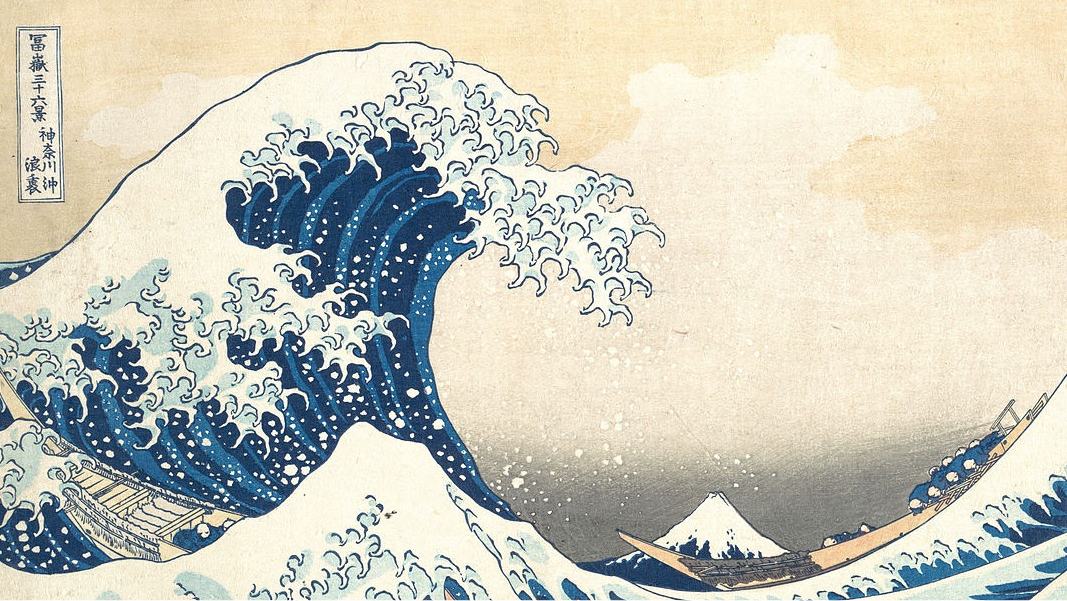
\includegraphics{img/kanagawa_16_9.png}
        }
    \end{center}
\end{frame}

% ------------------------------------------------------------------------------
\begin{frame}[allowframebreaks]{References}
    \printbibliography
\end{frame}
% ------------------------------------------------------------------------------


% ------------------------------------------------------------------------------
\appendix
% ------------------------------------------------------------------------------

\begin{frame}{Appendix Slide}\label{appendix1}
\begin{table}
    \caption{Summary Statistics}
    \label{appendix_summ_stat}
    \begin{adjustbox}{max width = \textwidth, width = 0.7\textwidth, center}
        \begin{threeparttable}
            \begin{tabular}{@{} lccccccc @{}} 
                \toprule
                Statistic & \multicolumn{1}{c}{N} & \multicolumn{1}{c}{Mean} & \multicolumn{1}{c}{St. Dev.} & \multicolumn{1}{c}{Min} & \multicolumn{1}{c}{Pctl(25)} & \multicolumn{1}{c}{Pctl(75)} & \multicolumn{1}{c}{Max} \\ 
                \hline \\[-1.8ex] 
                rating & 30 & 64.633 & 12.173 & 40 & 58.8 & 71.8 & 85 \\ 
                complaints & 30 & 66.600 & 13.315 & 37 & 58.5 & 77 & 90 \\ 
                privileges & 30 & 53.133 & 12.235 & 30 & 45 & 62.5 & 83 \\ 
                learning & 30 & 56.367 & 11.737 & 34 & 47 & 66.8 & 75 \\ 
                raises & 30 & 64.633 & 10.397 & 43 & 58.2 & 71 & 88 \\ 
                critical & 30 & 74.767 & 9.895 & 49 & 69.2 & 80 & 92 \\ 
                advance & 30 & 42.933 & 10.289 & 25 & 35 & 47.8 & 72 \\ 
                \bottomrule
            \end{tabular} 
            % Notes 
            \begin{tablenotes}
                \item \textit{Notes.} Using R base dataframe attitude.
            \end{tablenotes}
        \end{threeparttable}
    \end{adjustbox}
\end{table}
    
    \hyperlink{main1}{\beamergotobutton{Back to Main}}
\end{frame}
\end{document}
